\subsection{Caso d'uso UC6: Ricerca e selezione questionario esistente}
\label{UC6}
\begin{figure}[h]
\centering
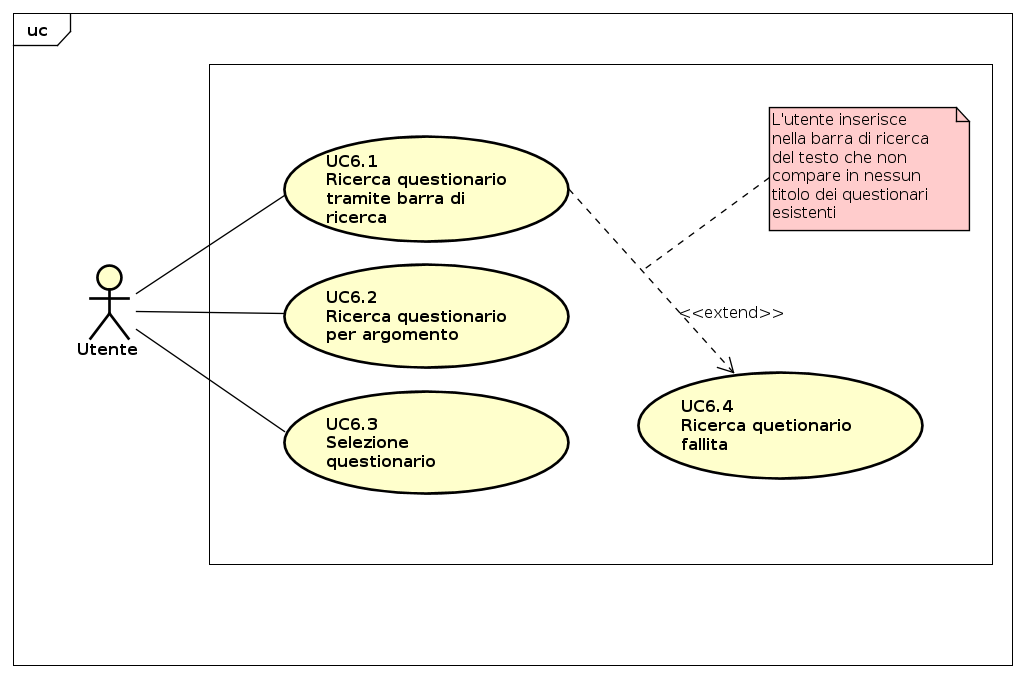
\includegraphics[scale=0.5,keepaspectratio]{UML/UC6.png}
\caption{UC6: Ricerca e selezione questionario esistente}
\end{figure}
\FloatBarrier
\begin{itemize}
\item\textbf{Attori Principali}: Utente non autenticato, Utente autenticato, Utente autenticato pro;
\item\textbf{Descrizione}: nella schermata principale qualsiasi utente che voglia svolgere un questionario può ricercarlo attraverso:
\begin{itemize}
\item la barra di ricerca;
\item una suddivisione per argomento dei questionari esistenti.
\end{itemize}
L'utente se è autenticato/autenticato pro può visualizzare nelle sue ricerche anche i questionari \textit{privati}. L'utente, per poter compilare un questionario, dovrà poi selezionare il questionario che ha scelto oppure potrà decidere di inserirlo nella lista ``Fai più tardi'';	
\item\textbf{Precondizione}: l'utente si trova nella pagina principale dell'applicazione;
\item\textbf{Postcondizione}: l'utente ha selezionato il questionario che vuole svolgere;
\item\textbf{Scenario principale}:
\begin{itemize}
\item L'utente cerca un questionario tramite barra di ricerca (UC6.1);
\item L'utente cerca un questionario per argomento (UC6.2);
\item L'utente seleziona il questionario \textit{pubblico} scelto (UC6.3);
\item L'utente autenticato/autenticato pro seleziona il questionario \textit{privato} scelto (UC6.4);
\item L'utente autenticato/autenticato pro aggiunge il questionario alla lista ``Fai più tardi''(UC6.5).
\end{itemize}
\item\textbf{Estensioni}: Ricerca questionario fallita (UC6.6).
\end{itemize}

\subsubsection{Caso d'uso UC6.1: Ricerca questionario tramite barra di ricerca}
\label{UC6.1}
\begin{itemize}
\item\textbf{Attori Principali}: Utente non autenticato, Utente autenticato, Utente autenticato pro;
\item\textbf{Descrizione}: all'interno della pagina principale dell'applicazione è presente una barra di ricerca dove è possibile cercare, attraverso il titolo, un determinato questionario;
\item\textbf{Precondizione}: l'utente si trova nella pagina principale dell'applicazione;
\item\textbf{Postcondizione}: l'utente visualizza i questionari che hanno nel titolo il testo che ha scritto nella barra di ricerca;
\item\textbf{Scenario principale}: l'utente utilizza la barra di ricerca per cercare un questionario del quale conosce il titolo o parte di questo.
\end{itemize}

\subsubsection{Caso d'uso UC6.2: Ricerca questionario per argomento}
\label{UC6.2}
\begin{itemize}
\item\textbf{Attori Principali}: Utente non autenticato, Utente autenticato, Utente autenticato pro;
\item\textbf{Descrizione}: all'interno della pagina principale dell'applicazione è presente una sezione contenete tutti i questionari esistenti suddivisi per argomento trattato;
\item\textbf{Precondizione}: l'utente si trova nella pagina principale dell'applicazione;
\item\textbf{Postcondizione}: l'utente visualizza un insieme di questionari suddivisi per argomento;
\item\textbf{Scenario principale}: l'utente che non conosce i questionari esistenti, si reca nella sezione in cui sono suddivisi per argomento in modo da rendere più facile la scelta di uno di questi. 
\end{itemize}

\subsubsection{Caso d'uso UC6.3: Selezione questionario pubblico}
\label{UC6.3}
\begin{figure}[h]
\centering
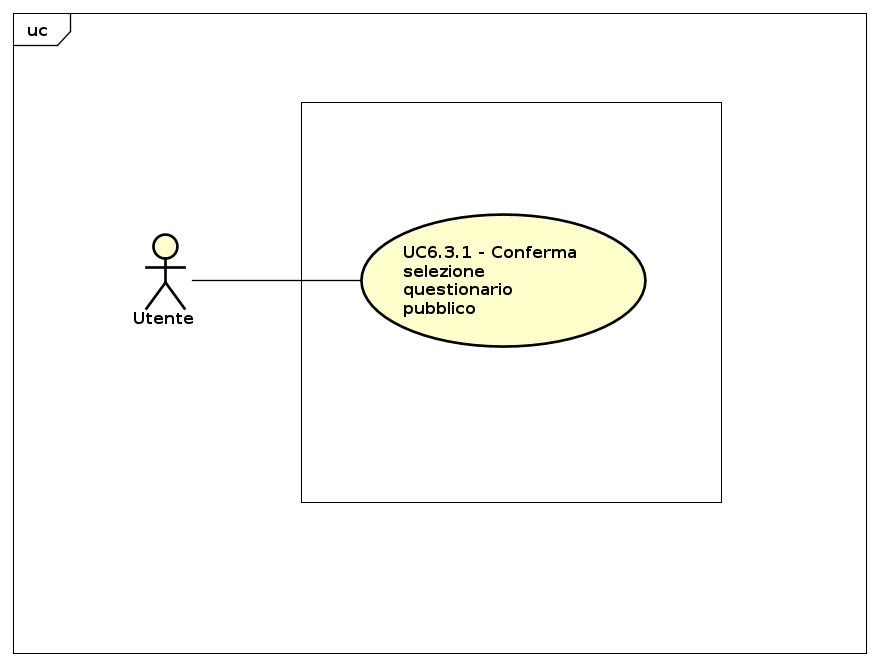
\includegraphics[scale=0.5,keepaspectratio]{UML/UC6_3.png}
\caption{UC6.3: Selezione questionario}
\end{figure}
\FloatBarrier
\begin{itemize}
\item\textbf{Attori Principali}: Utente non autenticato, Utente autenticato, Utente autenticato pro;
\item\textbf{Descrizione}: l'utente dopo aver scelto un questionario \textit{pubblico}, per iniziare a compilarlo, può selezionarlo;
\item\textbf{Precondizione}: l'utente ha scelto il questionario \textit{pubblico} che vuole svolgere;
\item\textbf{Postcondizione}: l'utente ha selezionato il questionario \textit{pubblico} scelto;
\item\textbf{Scenario principale}: l'utente conferma la selezione del questionario (UC6.3.1);
\item\textbf{Scenari alternativi}: l'utente cambia idea sul questionario \textit{pubblico} selezionato e annulla l'operazione tornando alla selezione dei questionari.
\end{itemize}

\subsubsection{Caso d'uso UC6.3.1: Conferma selezione questionario pubblico}
\label{UC6.3.1}
\begin{itemize}
\item\textbf{Attori Principali}: Utente non autenticato, Utente autenticato, Utente autenticato pro;
\item\textbf{Descrizione}: l'utente conferma la selezione del questionario, potendo così procedere con la compilazione;
\item\textbf{Precondizione}: l'utente ha selezionato un questionario \textit{pubblico};
\item\textbf{Postcondizione}: l'utente ha confermato la selezione del questionario;
\item\textbf{Scenario principale}: l'utente conferma di voler svolgere il questionario selezionato.
\end{itemize}

\subsubsection{Caso d'uso UC6.4: Selezione questionario privato}
\label{UC6.4}
\begin{figure}[h]
\centering
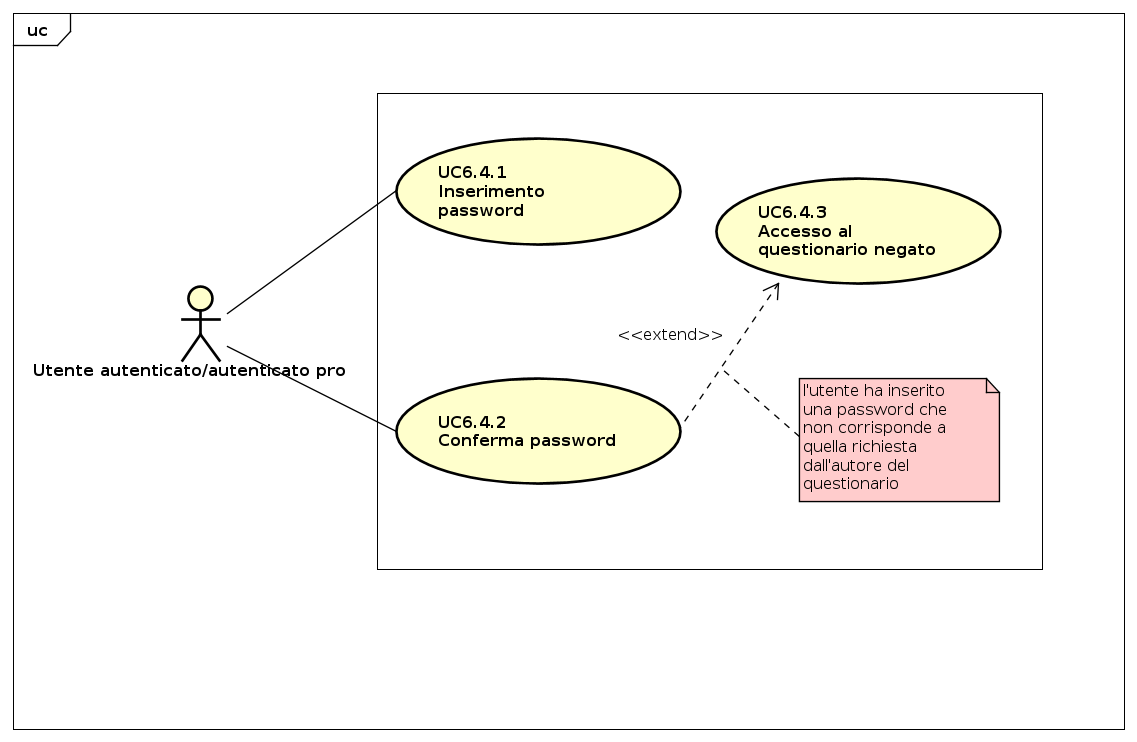
\includegraphics[scale=0.5,keepaspectratio]{UML/UC6_4.png}
\caption{UC6.4: Selezione questionario privato}
\end{figure}
\FloatBarrier
\begin{itemize}
\item\textbf{Attori Principali}: Utente autenticato, Utente autenticato pro;
\item\textbf{Descrizione}: l'utente può inserire la password richiesta dall'autore del questionario \textit{privato} e successivamente confermarla per poterlo compilare;
\item\textbf{Precondizione}: l'utente ha scelto il questionario \textit{privato} che vuole svolgere;
\item\textbf{Postcondizione}: l'utente ha selezionato il questionario \textit{privato} scelto;
\item\textbf{Scenario principale}:
\begin{itemize}
\item L'utente inserisce la password (UC6.4.1);
\item L'utente conferma l'inserimento della password (UC6.4.2).
\end{itemize}
\item\textbf{Estensioni}: Accesso al questionario negato (UC6.4.3);
\item\textbf{Scenari alternativi}: l'utente cambia idea sul questionario \textit{privato} selezionato e annulla l'operazione tornando alla selezione dei questionari.
\end{itemize}

\subsubsection{Caso d'uso UC6.4.1: Inserimento password}
\label{UC6.4.1}
\begin{itemize}
\item\textbf{Attori Principali}: Utente autenticato, Utente autenticato pro;
\item\textbf{Descrizione}: l'utente, per poter compilare il questionario, può inserire la password richiesta dal creatore di quest'ultimo;
\item\textbf{Precondizione}: l'utente ha selezionato un questionario \textit{privato};
\item\textbf{Postcondizione}: l'utente ha inserito la password;
\item\textbf{Scenario principale}: l'utente inserisce la password che gli consente di accedere al questionario.
\end{itemize}

\subsubsection{Caso d'uso UC6.4.2: Conferma password}
\label{UC6.4.2}
\begin{itemize}
\item\textbf{Attori Principali}: Utente autenticato, Utente autenticato pro;
\item\textbf{Descrizione}: l'utente può confermare la password inserita per poter accedere al questionario;
\item\textbf{Precondizione}: l'utente ha inserito la password;
\item\textbf{Postcondizione}: l'utente ha confermato la password inserita;
\item\textbf{Scenario principale}: l'utente conferma la password.
\end{itemize}

\subsubsection{Caso d'uso UC6.4.3: Accesso al questionario negato}
\label{UC6.4.3}
\begin{itemize}
\item\textbf{Attori Principali}: Utente autenticato, Utente autenticato pro;
\item\textbf{Descrizione}: l'utente ha inserito una password che non corrisponde a quella richiesta dall'autore del questionario, generando così un errore che gli impedisce di proseguire con la compilazione del suddetto fino a quando non verrà inserita la password corretta;
\item\textbf{Precondizione}: l'utente ha provato a confermare una password errata;
\item\textbf{Postcondizione}: il sistema avvisa l'utente dell'errore verificatosi tramite un opportuno messaggio;
\item\textbf{Scenario principale}: l'utente visualizza il messaggio di errore relativo alla password scorretta.
\end{itemize}

\subsubsection{Caso d'uso UC6.5: Aggiungi a ``Fai più tardi''}
\label{UC6.5}
\begin{itemize}
\item\textbf{Attori Principali}: Utente autenticato, Utente autenticato pro;
\item\textbf{Descrizione}: l'utente che sta cercando dei questionari da svolgere, può decidere di aggiungere alla personale lista ``Fai più tardi'' i questionari che sta visualizzando, potendoli recuperare così in seguito;
\item\textbf{Precondizione}: l'utente ha cercato dei questionari;
\item\textbf{Postcondizione}: l'utente ha aggiunto il questionario alla lista ``Fai più tardi'';
\item\textbf{Scenario principale}: l'utente che in quell'istante non può svolgere certi questionari che sta visualizzando, li può aggiungere alla personale lista ``Fai più tardi''.
\end{itemize}

\subsubsection{Caso d'uso UC6.6: Ricerca questionario fallita}
\label{UC6.6}
\begin{itemize}
\item\textbf{Attori Principali}: Utente non autenticato, Utente autenticato, Utente autenticato pro;
\item\textbf{Descrizione}: L'utente ha inserito nella barra di ricerca del testo che non compare in nessun titolo dei questionari esistenti;
\item\textbf{Precondizione}: l'utente ha utilizzato la barra di ricerca per cercare un questionario che non esiste;
\item\textbf{Postcondizione}: il sistema avvisa l'utente dell'errore verificatosi tramite un opportuno messaggio;
\item\textbf{Scenario principale}: l'utente visualizza un messaggio che lo avvisa del mancato ritrovamento di questionari.
\end{itemize}

